\documentclass[a4paper,american]{paper}
\usepackage[T1]{fontenc}
\usepackage[utf8]{inputenc}
\pagestyle{plain}
\usepackage{babel}
\usepackage{textcomp}
\usepackage{amsmath}
\usepackage{amsthm}
\usepackage{setspace}
\usepackage[unicode=true]{hyperref}
\usepackage{breakurl}
\usepackage{txfonts}
\usepackage{pxfonts}
\usepackage{tikz}

\graphicspath{ {./images/} }

\makeatletter
\providecommand*{\code}[1]{\texttt{#1}}
\makeatother

\begin{document}

\title{An interactive demonstration of counterfactual truth conditions%
	\footnote{Further title proposals:
		(B) Creating an educational computer game about counterfactuals in terms of a centered system of spheres
		(C) Implementing a computer game illustrating the truth conditions of counterfactuals as variably strict conditionals
	}
}

\subtitle{Proposal for a Bachelor Thesis (v0.1, 9 Juni 2022)}

\author{%
	Andreas Paul Bruno Lönne\\
	\code{\href{mailto:loenne@campus.tu-berlin.de}{loenne@campus.tu-berlin.de}}
}

\institution{
	Technische Universität Berlin\\discourse
	Degree program: Bachelor Informatik / Computer Science
}

\maketitle

\section*{Problem: An approachable showcase of counterfactuals}
{\it Counterfactuals} are in essence conditional statements carrying information about the relationship of a false {\it antedecent} and a {\it consequent}. Their truth value answers the question: ``If it were the case that A, would it then be the case that B?''. {\it Counterfactual~thought}---that is the thought of alternate outcomes---\cite{byrne_counterfactual_thought_2016} is common for humans to engage in and is consequently subject to a great volume of philosophical and mathematical discourse. 

Considering the amount of information available and the various propositions on how to mathematically model counterfactuals, gaining an understanding of the nuances of counterfactual truth conditions tends to be a difficult endeavour for any layman. I propose to remedy this issue by implementing a computer game based on a semantic game of counterfactuals.

\section*{Approach: A computer game on counterfactuals}
As part of my research I will try to find a didactically suitable semantic game for the evaluation of counterfactuals. More precisely I am looking to find a way to express {\it Lewis's formulation of counterfactual truth conditions} \cite{lewis_counterfactuals_1973} by way of a semantic game about proving counterfactual sentences.

I hope to create a software solution, that is intuitive and easy to use. The user is meant to be able to learn about counterfactuals, with little prior knowledge or time investment. Hence a minimalistic and functional user interface has to be developed.

For the purposes of visual clarity, usability and simplicity I intend to simplify the set of all accessible~worlds to a finite set of selected accessible exemplar~worlds and visualize them as shown in figure \ref{fig:closest_worlds}.

\begin{figure}[h]
	\centering
	\includegraphics[scale=0.5]{closest_worlds}
	\caption{graph representation of exemplar worlds}
	\label{fig:closest_worlds}
\end{figure}

Additionally i will determine an appropriate visual representation of counterfactual sentences from amongst various possibilities such as natural language, logical expressions and logical expression trees. While natural language is the most intuitive representation, it lacks the unambiguity of logical constructs and may create long unreadable sentences. Logical expressions, however, tend to be difficult to read and comprehend for laymen as well. Here are some examples of the same counterfactual statement expressed in different ways in (\ref{language}), (\ref{formula}) and figure \ref{fig:exptree}.

\begin{align}
    \text{\parbox{11cm}{``If Alexander~the~Great had not died at the age of 32 and attacked europe, the Romans would have defeated him''}}
     \label{language}
\end{align}
\begin{equation}
	(\neg\varphi_1\wedge\varphi_2)\boxright\psi
	\label{formula}
\end{equation}

\begin{figure}[h]
	\centering
	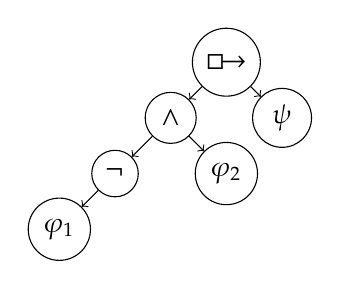
\begin{tikzpicture}[main/.style = {draw, circle}]
	\node[main] (1) {$\boxright$};
	\node[main] (2) [below left of=1] {$\wedge$};
	\node[main] (3) [below right of=1] {$\psi$};
	\node[main] (4) [below left of=2] {$\neg$};
	\node[main] (5) [below right of=2] {$\varphi_2$};
	\node[main] (6) [below left of=4] {$\varphi_1$};
	
	\draw[->] (1) -- (2);
	\draw[->] (1) -- (3);
	\draw[->] (2) -- (4);
	\draw[->] (2) -- (5);
	\draw[->] (4) -- (6);
	\end{tikzpicture}
	\caption{counterfactual sentence as a logical expression tree}
	\label{fig:exptree}
\end{figure}

It would also be desirable to find a way to convey the notions of {\it realism~about~possible~worlds} and {\it comparative~similarity}~between~worlds, since they may grant much greater insight into the meaning of counterfactuals.

In order to deliver an easily accessible software solution I intend to make use of the Phaser~3 Framework for Typescript to develop a web-application. Phaser~3 is well suited for this task because it is a lightweight framework, that fits the scope of the project and allows for distribution of the software with a small barrier to entry.

\section*{Schedule}

In accordance with \href{https://www.eecs.tu-berlin.de/fileadmin/f4/fkIVdokumente/StuPOs/Informatik/Lesefassung_BSc_Informatik.pdf}{StuPO~Bachelor~Informatik 2015}, the elaboration of the thesis is scheduled over a period of 20 weeks:
\begin{description}
\item [3 weeks] Familiarization with theory \& Game design.
\item [1 week] Implementation of a semantic game engine. (Output: Software)
\item [3 weeks] Implementation of the user interface. (Output: Counterfactual representation, Graph representation, Menu)
\item [2 weeks] Creation of levels or levelgenerator. (Output: Software)
\item [2 weeks] Testing \& QA.
\item [6 weeks] Write thesis. (Output: Thesis)
\item [3 weeks] Puffer
\end{description}

\section*{Thesis Outline (Sketch)}

\begin{enumerate}
	\item Introduction
	\begin{enumerate}
		\item Problem description
		\item Context / related work
		\item Overview
	\end{enumerate}
	\item Formulation of the semantic game of counterfactuals
	\item Implementation
	\begin{enumerate}
		\item Design decisions (visual Representation of cfs, ...)
		\item Framework
		\item Concrete implementation of the semantic game engine
		\item Evaluation of the implementation
	\end{enumerate}
	\item Conclusion
	\begin{enumerate}
		\item Summary
		\item Outlook
	\end{enumerate}
\end{enumerate}

\bibliographystyle{alphaurl}
\nocite{*}
\bibliography{expose}

\end{document}
